Activities were created to occupy the enterire screen and that's 
ok for small devices, but for large devices such as tablets,
we could use the space in a better way. 

Fragments can be seen as sub-activities, as they may respond to back-buttons 
and have their own \textbf{life-cycle}. However, a fragment lifecycle is 
related to the activity lifecycle. 
One activity can have many fragments and the point is that they all use the same 
thread (the main one).

\subsection{Fragment Lifecycles}

\begin{figure}[h]
\centering
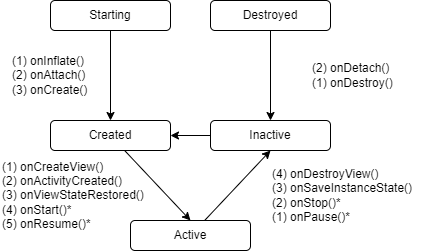
\includegraphics[width=0.8\linewidth]{figures/03_fragment_state_diagram.png}
\caption{Fragment State Diagram}
\label{fig:fragment_state_diagram}
\end{figure}


Now let's explain the sequence of commands called in a fragment life-cycle. 
\begin{itemize}
\item \texttt{onInflate(activity: Activity, attrs: AttributeSet, savedInstanceState: Bundle) }: Called in 
the beggining of the activity, when the fragment sets its content layout. The AttributeSet contains the attributes defined in the activity layout. They should be
parsed and saved. The fragment is not yet attached to the activity.

\item \texttt{onAttach(activity: Activity)}: Now the activity is attached to the fragment. In other words, 
it's possible to get the activity with the function \texttt{getActivity()} inside the fragment. 
It's also possible to get the arguments with \texttt{getArguments()}, but only the arguments set until
this moment.

\item \texttt{onCreate(savedInstanceState: Bundle)}: \textbf{It's when the fragment starts the process 
of creation} called at the beginning of the owner activity onCreate() callback. Usually, the 
\textbf{activity View hierarchy is not yet inflated}. You can create here another thread to do 
lengthy data loading operations.

\item \texttt{onCreateView(inflater: LayoutInflater, container: ViewGroup, savedInstanceState: Bundle)}:
This function should return the inflated View of this fragment. If the container is null, then null
must be returned. The container is the ViewGroup in the activity layout that will display the fragment.
Do not attach the fragment to this container. Some specialized fragments (e.g., ListFragment) do not need 
this callback.

\item \texttt{onActivityCreated(savedInstanceState: Bundle)}: here the onCreate() method of the activity 
is now complete. The complete interface is now built, including other present fragments. 

\item \texttt{onStart() and onResume()}: tied with the activity corresponding callbacks.

\item \texttt{onPause()}: the first to be called (the fragment can be put on the fragment back stack). You
should stop playing sounds, related to this fragment, here.

\item \texttt{onStop()} : tied with the onStop() callback of the activity. A stopped fragment can go straight
to the onStart() callback.

\item \texttt{onDestroyView()}: when the fragment is being killed or saved, this will be called. Here its View
hierarchy is already detached from the activity layout.

\item \texttt{onDestroy()}: is called when the fragment is no longer in use (but still existing in the activity).

\item \texttt{onDetach()}: here the fragment does not belong anymore to the activity and the interface
resources are already freed.

\item \texttt{onSaveIntanceState(outstate: Bundle)}: called somewhere before onDestroy(). It should save
internal state in the provided Bundle. That Bundle is passed to the entry callbacks.

\end{itemize}

\subsection{Fragment creation}

The fragment creation can be \textbf{STATIC} or \textbf{DYNAMIC}.

\begin{itemize}
    \item \textbf{STATIC}: Whenever the activity inflates its layout and has a <fragment> element in it, 
    the system constructs the Fragment
    \item \textbf{DYNAMIC}: If Fragments are built in the code, then a static factory method must be created in the fragment 
    class. It's recommended to have a factory for the fragment, since fragments doesn't have a constructor.
\end{itemize}

\begin{lstlisting}[title=Fragment Factory]
fun MyFragment newInstance(index: Int) {
    val f = MyFragment()
    val args = Bundle() 
    args.putInt("index", index)
    f.arguments = args
    return f
}
\end{lstlisting}

\begin{tcolorbox}[title=Bundled arguments]
    The arguments for a fragment inialization must be received in the factory must be passed as parameter
and then \textit{Bundled}. Bundled arguments are \textbf{preserved in the rotation} and are available as 
property.
\end{tcolorbox}

\subsection{Fragment Manager (supportFragmentManager)}
Activities and fragments can manager other active fragments. This can be done by using the 
\texttt{FragmentManager} object. This object is available at the property \texttt{supportFragmentManager}. 

It can:
\begin{itemize}
    \item Find fragments
    \item Manipulate the fragment back stack
    \item Save and restore references to fragments and fragment internal state
    \item Add, replace, remove, hiding and showing can be done and must be executed as a transaction.   
\end{itemize}

Example:

\begin{lstlisting}[title=Fragment transaction]
    /**
     * Changes the view to a fragment that shows the items inside the history.
     */
    private fun changeToBasketHistoryProducts(){
        val basketHistoryProducts = BasketHistoryProducts.newInstance(intent.extras!!)
        val fragmentManager = this.supportFragmentManager
        val fragmentTransaction = fragmentManager.beginTransaction()    // Starting transaction.
        fragmentTransaction.add(android.R.id.content, basketHistoryProducts)
        fragmentTransaction.commit()    // Should end with commit

    }
\end{lstlisting}

\subsection{Implementing a fragment}

\begin{lstlisting}[title=Fragment implementation]
    // In the parent activity
    class ParentActivity : AppCompatActivity() {  
      override fun onCreate(savedInstanceState: Bundle?) {  
        super.onCreate(savedInstanceState)  
        
        val frag = MyFragment.newInstance(intent.extras!!)  
        ... 
      }
      ...
    } 
     
    // In the Fragment class
    class MyFragment : Fragment() {
      var mIndex = 0;  
      
      override fun onCreate(savedInstanceState: Bundle?) {  
        super.onCreate(savedInstanceState)  
        mIndex = arguments?.getInt("index") ?: 0  
      }
        
      override fun onCreateView(inflater: LayoutInflater, container: ViewGroup?, savedInstanceState: Bundle?): View? {  
        if (container == null)  
          return null  
          
        // Don't tie this fragment to anything through the inflater
        val v = inflater.inflate(R.layout.details, container, false) 
        v.findViewById<TextView>(R.id.text1).text = Planets.PROPS[mIndex]  
        return v  
      }  
      
      // Fragment factory
      companion object {  
        @JvmStatic
        fun MyFragment newInstance(index: Int) { 
          val f = MyFragment() 
          val args = Bundle()
          args.putInt("index", index) 
          f.arguments = args 
          return f 
        }
      }
    }
    
\end{lstlisting}

\textbf{NOTE}: The method of building dialogs from the Dialog class doesn't take care 
automatically of lifecycle events, like the destruction and re-creation. You should embed the 
\texttt{DialogFragment}. 



